% Sample file on how to use subfiles.
\documentclass[ExampleMasters.tex]{subfiles}

\begin{document}

\chapter{Introduction}

\chapter{Theory}
\section{Macroscopic modeling}

\section{Fine-scale problem}
\subsection{Mixed velocity-pressure formulation}
\subsection{Surface tension}


\chapter{Variationally Consistent Homogenization}














\section{The process of sintering of hardmetal}

Manufacturing of PM products is based on the ``welding'' (sintering) of particles due to heating or combined heating and mechanical loading (uniaxial or isotropic pressing).
To model and simulate the sintering of hard metals, typically WC with Co as the binder metal in the case of a WC-Co-Ti-C system, is particularly challenging in view of the fact that the sintering process involves both solid and melt states of the constituents.
In brief, the manufacturing process can be split into three different sequential stages:
(I) Compaction of powder compound, with initially around \SI{70}{\percent} porosity, into a ``green body'' with roughly \SIrange{20}{40}{\percent} porosity.
(II) Heating in oven up well above the melting temperature for Co (ca \SI{1500}{\celsius}).
(III) Cooling to room temperature.

The purpose is to achieve net-shape already of the green body, whereby the subsequent sintering would result mainly in change of volume (without distortion, i.e. shear deformation).
Since uniaxial pressing is normally used for the initial compaction of hard metal, it is likely that wall friction leads to inhomogeneous
distribution of residual stresses and bulk density in the green body (at least to some extent).
This is an unwanted effect that obscures the goal of net-shape.

During the heating phase, thermal expansion is combined with a certain amount of solid state sintering before melting of the binder, which is necessary in order to achieve ``liquid-phase'' sintering.
During the hold-time at the given temperature, significant compaction (densification, consolidation) takes place due to a combination of solid deformation, diffusion and liquid motion, which brings about reduced porosity.
The so-called ``sintering stress'', which is a macro-scale manifestation of the surface tension between the constituents and the pores, is the ``driving force'' for compaction; hence, sintering can take place under zero external load of the specimen (known as ``free sintering'').
However, the residual stresses after compaction will effect the process.

\textbf{Remark:} It is possible to achieve a sintered product below or above the melting temperature of the Co-binder.
Up to \SI{80}{\percent} of the densification can be achieved in pure solid state sintering, although a completely dense product can only be achieved with liquid phase.
These two cases are often denoted solid and liquid state sintering, respectively, in the literature.

% There are generally two characteristic stages in terms of porosity characteristics:
% At the early stage of sintering all pores are connected, which leads to quite rapid densification, in particular due to viscous flow of the liquid binder. Later on, within a certain temperature interval, all binder has solidified and the (possibly remaining) pores are closed off (and isolated) into near-equilibrium, which leads to much lower rate of consolidation.

Clearly, the aim of the process is that the final product is completely dense, i.e. there is no rest-porosity, with no net-shape distortion.
This may be hard to accomplish if the green body bulk density is severely inhomogeneous and/or the liquid phase sintering is inefficient (in terms of insufficient amount of binder phase and/or incomplete melting).

\section{Modeling and simulation efforts --- A brief review}

A wealth of literature deals with the modeling and simulation of the sintering process.
Primarily, this relates to the constitutive modeling of
(1) the powder material response for green body (pre)compaction and 
(2) the high temperature response and sintering mechanisms pertinent to both solid and liquid phase sintering.
Modeling efforts can be classified by two major paradigms: \emph{a priori macroscale modeling} and \emph{micromechanics modeling and computational homogenization}.

\subsection{Macroscale modeling}

A vast majority of the existing literature on \emph{a priori} macro-scale modeling is devoted to the compaction stage, and it is noted that very few (if any) attempts have been made to develop a unifying macroscopic constitutive model for the compaction and sintering stages.
As to the compaction process, material rate-independence (elasto-plasticity) is a common (and valid) assumption.
Such plasticity models are often taken, at least conceptually, from soil mechanics.
The major focus is on the evolution of the yield surface due to changing porosity as the predominant hardening mechanism, e.g.\ Fleck et al. \cite{FleKuhMcM1992},
Oliver et al. \cite{OliOllCan1996}, Brandt and Nilsson \cite{BraNil1998}, Redanz \cite{Red1998}, Kraft \cite{Kra2003}.

For the solid phase sintering, the major feature is the strong rate-dependence close to, and above, the melting temperature of the binder.
Models based on viscoelasticity and viscoplasticity have, therefore, been proposed to simulate the creep behavior of the highly deformable (and even partly melt) binder, e.g. Shinigawa \cite{Shi1996}, Brandt and Nilsson \cite{BraNil1998}.
Clearly, it is of utmost importance to model the high sensitivity of yield stress to temperature, e.g. Mähler et al. \cite{MahEkhRun2001a}.
The task of providing a rational thermodynamic definition of the sintering stress was addressed by, e.g. Reid and Oakberg \cite{ReiOak1990}, Mähler and Runesson \cite{MahRun2000}.

As to liquid phase sintering, the text-book by German \cite{Ger1985} is still an authority in the field.
Examples of the rich literature are Svoboda et al. \cite{SvoRieGae1996}, Xu and Mehrabahdi \cite{XuMeh1997}, Lu et al. \cite{LuXuYiGer2001}, who used a single-phase approach.
To date, it seems that no attempts have been made in the literature to use mixture theory, which explicitly acknowledges the coexistence of a solid skeleton of the WC-particles and partly solidified and liquid Co.

\subsection{Micromechanics modeling and computational homogenization}

Most micromechanically based models consider idealized geometrical arrangement, such as a regular array of (in many cases only two) spheres, within a Representative Volume Element (RVE).
One common approach is to consider grain boundary diffusion, e.g. Helle, et al. \cite{HelEasAsh1985}, McMeeking and Kuhn \cite{McMKuh1992}, Riedel and Svoboda \cite{RieSvo1993} and Shinigawa \cite{Shi1996} and particle bridging via diffusion, e.g. Svoboda and Riedel \cite{SvoRie1995}, Binet \cite{BinLenHeaGer2004}, Luque et al. \cite{LuqAldMarMarSevFar2005}, as the principal mechanisms for densification.
Some attempts have been made too include more realistic microstructural arrangements and carry out computational homogenization to obtain response functions, e.g. Mähler and Runesson \cite{MahRun2000}.

Early attempts to numerically simulate the surface-tension driven reshaping of contacting particles are by Jagota and Dawson \cite{JagDaw1988a,JagDaw1988b} and van de Vorst \cite{Vorst1993}.
In a series of papers, Zhou and Derby \cite{ZhoDer1998,ZhoDer2001} emphasize efficient finite element algorithms to trace the complex 3-dimensional flow of multi-particle interaction.
The main challenges  are the complex subscale geometry and the moving free boundary giving rise to very large deformations and severe topology changes.
Recent developments of free-boundary tracing FE-strategies for large deformations (without severe topological changes) are discussed by Peric and coworkers, \cite{DetPer2006}, \cite{SakPer2006a}, \cite{SakPer2006b}.
All the mentioned work consider surface tension effects in fluids.
A recent extension to include surface tension in the context of solid modeling, where anisotropic surface energy may be present, is due to Javili and Steinmann \cite{JavSte2010:3d}.

Micro-mechanical analysis must be accompanied by computational homogenization in order to obtain a predictive model for a component.
One possibility is socalled upscaling, i. e. to use the subscale modeling to calibrate a macroscopic model.
A more appealing, but theoretically and computationally more challenging, possibility is to carry out full-fledged simultaneous coupling between the micro- and macro-scales, which is known as Computational Multiscale Modeling (CMM), or the FE\textsuperscript{2} strategy.
This is certainly the current international trend in material modeling for engineering purposes; however, to our knowledge no work on the fully coupled FE\textsuperscript{2} applied to the sintering problem has been published (at least not in main-stream journals).

\chapter{Aim and Scope of Research}

The thesis concerns the development of a predictive tool for the computational modeling of sintering of hardmetal, that involves a liquid (melt binder) phase.
Virtually all modeling in the literature aiming for quantitative predictions on the engineering scale is based on \emph{a priori} homogenized macroscopic material models.
In this Ph.D.\ project (of which the present licentiate thesis represents the first part), the relevant equations are obtained via micromechanical modeling and computational homogenization.

The main purpose and specific aims of the Ph.D. project are two-fold:
\begin{itemize}
\item To establish a computational model for the prediction of final shape (distortion), residual stresses and remaining porosity in sintered hardmetal products.
Particular emphasis is placed on the role of liquid phase sintering, e.g. with respect to the amount and composition of the (melt) binder metal, size distribution of particles, etc.

\item To calibrate and validate the constitutive models using data from the literature and from present and past collaborators.
Experimental data from component tests are available from a previous joint research project with Swedish partners.
\end{itemize}
In order to achieve this goal, the following tasks are identified in the present licentiate thesis:
\begin{itemize}
 \item Develop the micro-mechanical relations for an ideal setting of viscous particles in contact that sinter due to surface tension.
 \item Use computational homogenization and a fully coupled FE\textsuperscript{2} strategy to obtain a predictive model.
 \item Develop FE-software, in particular for efficient implementation of parallel algorithms.
\end{itemize}

\chapter{Modeling Features}
%%%%%%%%%%%%%%%%%%%%%%%%%%%%%%%%%%%%%%%%%%%%%%%%%%%%%%%%%%%%%%%%%%%%%%%%%%%%%%%%%%%%%%%%%%%%%%%%%%%%%%%%%%%
\section{Constitutive modeling of constituents}
Elastic deformation is neglected in the subscale constituents, which is a reasonable assumption since the (visco)plastic deformation is totally dominating the process.
With plastic incompressibility, this leads to an isotropic incompressible Stokes flow within the particles.
The chosen constitutive model is potentially nonlinear and the stress deviator $\ts\sigma_\dev$ is proportional the deviatoric strain rate $\ts d_\dev$:
\begin{equation}
    \ts{\sigma}_\dev(\ts{d}) = 2\tilde{\mu}\ts{d}_\dev, \quad
    \tilde{\mu}\defeq \frac{\sigma_\eqv}{3d_\eqv}
    %\frac{\mu}{1+\frac{3\mu k\left(\sigma_\eqv\left(d_\eqv\right)\right)}{\sigma_\eqv\left(d_\eqv\right)}}
%\label{eq203}
\end{equation}
Thermal expansion is not yet considered, which means that the process is assumed to take place after initial heating.

It is worth noting that, even though the subscale constituents are incompressible, the macroscopic change is compressible due to shrinking pores within the RVE's. The macroscopic response of a given specimen will eventually be partially incompressible at the later stages of sintering. 
In \refpaper{B}, the problem of incompressible RVE's is dealt with.

In the absence of acceleration, the balance equations for the quasi-static motion of the viscoplastic particles can be established in the spatial setting as follows:
%-----------------------------------------------------------------
\begin{subequations}\label{eq:stokesflow}
\begin{align}
    -\ts{\sigma}\cdot\diff & = \ts{0} \quad% \mbox{ in }\Omega^\particle \defeq \cup_i \Omega^\particle_i
\label{eq:stokesflow_momentum}
\\
    \ta{v}\cdot\diff & = 0 \quad% \mbox{ in }\Omega^\particle
\label{eq:stokesflow_continuity}
\end{align}
\end{subequations}
Note that these equations are intrinsic to the particles.

%%%%%%%%%%%%%%%%%%%%%%%%%%%%%%%%%%%%%%%%%%%%%%%%%%%%%%%%%%%%%%%%%%%%%%%%%%%%%%%%%%%%%%%%%%%%%%%%%%%%%%%%%%%
\section{Surface tension}

\begin{figure}[th!]
    \centering
    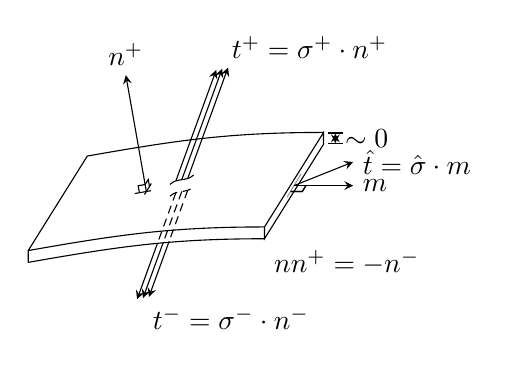
\begin{tikzpicture}[>=stealth,scale=1.5]
 \coordinate (A) at (0,0);
 \coordinate (B) at (2,0.2);
 \coordinate (C) at (2.5,1);
 \coordinate (D) at (0.5,0.8);
 \coordinate (At) at (0,-0.1);
 \coordinate (Bt) at (2,0.1);
 \coordinate (Ct) at (2.5,0.9);

 \draw (A) to[out=10,in=180] (B)
      (At) to[out=10,in=180] (Bt)
      (Bt) -- (B) -- (C) coordinate[midway] (E) -- (Ct) -- cycle
      (At) -- (A) -- (D) to[out=10,in=180] (C);

 % Binormal m
 \draw[draw=black!40] (E)++(0,-0.05)++(-0.06,-0.1) -- +(0.12,0.2);
 \draw[->] (E)++(0,-0.05) -- +(0.5,0) node[right]{$\ta{m}$};
 \draw[->] (E)++(0,-0.05) -- +(0.5,0.2) node[right]{$\hat{\ta{t}}=\hat{\ts{\sigma}}\cdot\ta{m}$};
 \draw (E)++(-0.03,-0.1) -- ++(0.1,0) -- +(0.03,0.05);
 \draw (E)++(0,-0.05)++(-0.03,-0.05) -- ++(0.1,0) -- +(0.03,0.05);

 
 % Normal
 \coordinate (n) at (1,0.5);
 \draw[->] (n) -- +(100:1) node[above]{$\ta{n}^+$};
 \draw (n)++(190:0.06) -- ++(100:0.06) -- +(190:-0.06);
 \draw (n)++(190:0.1) -- +(190:-0.14);
 \draw (n)++(58:0.05) -- ++(100:0.06) -- +(58:-0.05);
 \draw (n)++(58:0.08) -- +(58:-0.11);
 %\draw (n)++(190:0.06) -- ++(58:0.05) -- ++(190:-0.06);
 
 % Traction +
 \draw[->] (1.3,0.6) -- +(70:1) node[above right]{$\ta{t}^+ = \ts{\sigma}^+\cdot\ta{n}^+$};
 \draw[->] (1.35,0.61) -- +(70:1);
 \draw[->] (1.25,0.59) -- +(70:1);
 \draw (1.2,0.56) to[out=45,in=-135] (1.4,0.64);

 % Traction -
 \draw[densely dashed] (1.3,0.5) -- +(-110:0.46) coordinate (tmin); \draw[->] (tmin) -- +(-110:0.5) node[below right]{$\ta{t}^- =  \ts{\sigma}^-\cdot\ta{n}^-$};
 \draw[densely dashed] (1.35,0.51) -- +(-110:0.46) coordinate (tmin); \draw[->] (tmin) -- +(-110:0.5);
 \draw[densely dashed] (1.25,0.49) -- +(-110:0.46) coordinate (tmin); \draw[->] (tmin) -- +(-110:0.5);
 \draw[densely dashed] (1.2,0.46) to[out=45,in=-135] (1.4,0.54);

 % Thickness
 \draw[|<->|] ([xshift=0.1cm]C) -- ([xshift=0.1cm]Ct) node[midway,right] {$\sim 0$};

 % Definition
 \node[right] at (2,-0.1) {$\ta{n} \defeq \ta n^+ = -\ta n^-$};
\end{tikzpicture}
    \caption{Thin shell representing a surface with in-plane forces due to ``surface tension''.}
    \label{fig:surfacestress}
\end{figure}
A vital part of the simulation is the modeling of surface tension which acts as the ``driving force'' for liquid-phase sintering.
An extensive theory on boundary energy potentials has been developed by Steinmann \cite{Steinmann2008:boundaryenergies}, which has served as the basis for the surface tension modeling in this work.
In short; equilibrium across a surface $\Gamma$ represented by a thin shell bounded by the curve $\mathcal{C}$, as in Figure~\ref{fig:surfacestress} can be stated as:
\begin{align}
    \ta{t}^+ + \ta{t}^- + \ta{t}_\surf &= \ta{0} \quad \mbox{on} \,\, \Gamma \quad \mbox{with } \ta{t}_\surf \defeq \hat{\ts\sigma}\cdot\hat{\diff}
\label{eq103KR}\\
    \sum_i \hat{\ta t}_i &= \ta{0} \quad \mbox{on} \,\, \mathcal{C}
\label{eq104KR}
\end{align}
where $\hat\diff \defeq \diff - (\diff\cdot\ta n)\ta n$.
For an isotropic surface potential one obtains, $\hat{\ts\sigma} = \gamma_\surf(\ts I-\ta n\outerp\ts n)$, and the common expression for the surface traction representing surface tension is obtained:
\begin{align}
 \ta t_\surf = -\kappa \gamma_\surf \ta n,\quad \text{where}\quad \kappa \defeq \ts n\cdot\hat\diff
\end{align}
where $\kappa$ is the curvature.


%%%%%%%%%%%%%%%%%%%%%%%%%%%%%%%%%%%%%%%%%%%%%%%%%%%%%%%%%%%%%%%%%%%%%%%%%%%%%%%%%%%%%%%%%%%%%%%%%%%%%%%%%%%
\section{RVE-problem}
\begin{figure}[th!]
  \centering
  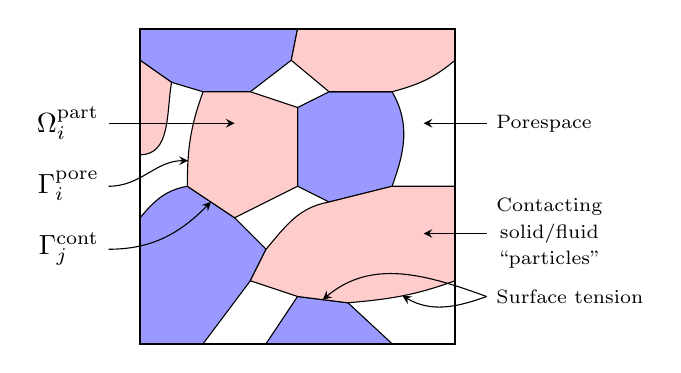
\begin{tikzpicture}[>=stealth,scale=4]
  \coordinate (A) at (0.35,0.2);
  \coordinate (B) at (0.4,0.3);
  \coordinate (C) at (0.3,0.4);
  \coordinate (D) at (0.15,0.5);
  \coordinate (E) at (0.66,0.13);
  \coordinate (F) at (0.6,0.45);
  \coordinate (G) at (0.8,0.5);
  \coordinate (H) at (0.5,0.5);
  \coordinate (I) at (0.5,0.75);
  \coordinate (J) at (0.6,0.8);
  \coordinate (K) at (0.8,0.8);
  \coordinate (L) at (0.35,0.8);
  \coordinate (M) at (0.5,1);
  \coordinate (N) at (0,0.9);
  \coordinate (O) at (0.1,0.83);
  \coordinate (P) at (0.5,0.15);
  \coordinate (Q) at (0.48,0.9);
  \coordinate (R) at (0.2,0.8);
  
  % Region 1 particles 
  \draw[fill=blue!40] 
  (0,0) -- (0.2,0) -- (A) -- (B) -- (C) -- (D) to[out=190,in=50] (0,0.4) -- cycle %A
  (0.4,0) -- (P) -- (E) -- (0.8,0) -- cycle %B
  (F) -- (G) to[out=70,in=-60] (K) -- (J) -- (I) -- (H) -- cycle %C
  (M) -- (Q) -- (L) -- (R) -- (O) -- (N) -- (0,1) -- cycle %D
  ;

  % Region 2 particles
  \draw[fill=red!20]
  (0,0.6) to[out=0,in=-100] (O) -- (N) -- cycle %E
  (D) to[out=90,in=-110] coordinate[near start] (surf3) (R) -- (L) -- (I) -- (H) -- (C) -- (D) coordinate[midway] (surf4) %F
  (M) -- (Q) -- (J) -- (K) to[out=15,in=-140] (1,0.9) -- (1,1) -- cycle %G
  (1,0.2) to[out=-160,in=5] coordinate[midway] (surf1) (E) -- (P) coordinate[midway] (surf2) -- (A) -- (B) to[out=50,in=-170] (F) -- (G) -- (1,0.5) -- cycle %H
  ;

  \draw[thick] (0,0) rectangle (1,1);

  % Annotations
  \draw[<-] (0.9,0.7) -- (1.1,0.7) node[right,font=\scriptsize] {Porespace};
  \draw[<-] (0.9,0.35) -- (1.1,0.35) node[right,font=\scriptsize] {\shortstack{Contacting\\solid/fluid\\``particles''}};
  \draw[<-] (surf1) to[out=-30,in=-160] (1.1,0.15) node[right,font=\scriptsize] {Surface tension};
  \draw[<-] (surf2) to[out=40,in=160] (1.1,0.15); % extra arrow
  \draw[<-] (surf3) to[out=180,in=0] (-0.1,0.5) node[left] {$\Gamma_i^{\mathrm{pore}}$};
  \draw[<-] (surf4) to[out=-135,in=0] (-0.1,0.3) node[left] {$\Gamma_j^{\mathrm{cont}}$};
  \draw[<-] (0.3,0.7) to[out=180,in=0] (-0.1,0.7) node[left] {$\Omega_i^{\mathrm{part}}$};
\end{tikzpicture}
  \caption{Microstructure of porous particulate material with sintering particles in contact.}
  \label{fig:micro}
\end{figure}
The fundamental microconstituents of the subscale are defined in Figure~\ref{fig:micro}.
Surface tension could be considered on all boundaries; $\Gamma_i^{\mathrm{pore}}$ and $\Gamma_j^{\mathrm{cont}}$; however, it is assumed to be zero on $\Gamma_j^{\mathrm{cont}}$ in all the numerical examples in the appended papers.
%
\begin{figure}[H]
    \centering
    \begin{tikzpicture}[>=latex,scale=2] % Use this to scale the image. Text is always normal-size
  \def\particleradius{1.05} % Adjust this to change the contact size.
  \pgfmathsetmacro{\contactsize}{sqrt(\particleradius^2-1)} % Automatically calculated.
  \begin{scope}[very thick]
  	\draw[clip] (-1,-1) rectangle (1,1);
  	\draw[clip]
  		(-1,-1) circle (\particleradius)
 		( 1,-1) circle (\particleradius)
 		(-1, 1) circle (\particleradius)
   		( 1, 1) circle (\particleradius);
  	\fill[fill=black!10] (-1,-1) rectangle (1,1);
  \end{scope}
  % Markers
  \foreach \q in {0,90,180,270} { \draw[rotate=\q] (1-\contactsize,-0.05) -- +(0,0.1); }
  \draw[dashed,gray] (-1.1,0) -- (1.1,0) (0,-1.1) -- (0,1.1);
  % Annotations
  %\node[below] at (0,0) {$\Omega_\Box^p(0)$};
  \draw[|<->|] (-1,-1.4) -- (1,-1.4) node[midway,above] {$L_\Box(0)$};
  \draw[<->|] (-1,-0.05) -- +(\contactsize,0) node[midway,below] {$a_0$};
  \node at (0.6,-0.6) {$\Omega_\Box^{\mathrm{part}}(0)$};
  \draw[<-] (1,-0.5) -- +(0.2,0) node[right] {$\Gamma_\Box(0)$};
  \draw[<-] (1,1) ++(-135:\particleradius) -- +(0.00,0.15) node[above right] {$\Gamma_\Box^{\mathrm{pore}}(0)$};
  
  %\draw[use as bounding box] (-1.7,-1.5) rectangle (1.7,1.1);
  %\useasboundingbox (-1.7,-1.5) (1.7,1.1);
  % Transformation arrow (makes the picture very unaligned)
  %\draw[->] (1.5,0) to[out=45,in=-150] (2,0);% +(135:0.1) -- (2,0) -- +(-135:0.1);
\end{tikzpicture}

    %\subfloat[$t = 0$]{\begin{tikzpicture}[>=latex,scale=2] % Use this to scale the image. Text is always normal-size
  \def\particleradius{1.05} % Adjust this to change the contact size.
  \pgfmathsetmacro{\contactsize}{sqrt(\particleradius^2-1)} % Automatically calculated.
  \begin{scope}[very thick]
  	\draw[clip] (-1,-1) rectangle (1,1);
  	\draw[clip]
  		(-1,-1) circle (\particleradius)
 		( 1,-1) circle (\particleradius)
 		(-1, 1) circle (\particleradius)
   		( 1, 1) circle (\particleradius);
  	\fill[fill=black!10] (-1,-1) rectangle (1,1);
  \end{scope}
  % Markers
  \foreach \q in {0,90,180,270} { \draw[rotate=\q] (1-\contactsize,-0.05) -- +(0,0.1); }
  \draw[dashed,gray] (-1.1,0) -- (1.1,0) (0,-1.1) -- (0,1.1);
  % Annotations
  %\node[below] at (0,0) {$\Omega_\Box^p(0)$};
  \draw[|<->|] (-1,-1.4) -- (1,-1.4) node[midway,above] {$L_\Box(0)$};
  \draw[<->|] (-1,-0.05) -- +(\contactsize,0) node[midway,below] {$a_0$};
  \node at (0.6,-0.6) {$\Omega_\Box^{\mathrm{part}}(0)$};
  \draw[<-] (1,-0.5) -- +(0.2,0) node[right] {$\Gamma_\Box(0)$};
  \draw[<-] (1,1) ++(-135:\particleradius) -- +(0.00,0.15) node[above right] {$\Gamma_\Box^{\mathrm{pore}}(0)$};
  
  %\draw[use as bounding box] (-1.7,-1.5) rectangle (1.7,1.1);
  %\useasboundingbox (-1.7,-1.5) (1.7,1.1);
  % Transformation arrow (makes the picture very unaligned)
  %\draw[->] (1.5,0) to[out=45,in=-150] (2,0);% +(135:0.1) -- (2,0) -- +(-135:0.1);
\end{tikzpicture}
\label{fig:4particle_rve_a}}
    %\subfloat[$t > 0$]{\begin{tikzpicture}[>=latex,scale=1.6] % Use this to scale the image. Text is always normal-size
  \def\particleradius{1.05} % Adjust this to change the contact size.
  \draw[thick,fill=black!10,even odd rule] (0.9,-1.1) 
  	to[out=190,in=10] (-1.1,-0.9)
  	to[out=80,in=-110] (-0.9,1.1)
  	to[out=10,in=-160] (1.1,1.1)
  	to[out=-100,in=60] (0.9,-1.1) -- cycle
  	(-0.1,-0.5) to[out=180,in=-45] (-0.2,-0.15) to[out=135,in=-90]
  	(-0.5,0)    to[out=90,in=-135] (-0.15,0.15)  to[out=45,in=-180]  
  	(0.1,0.5)   to[out=0,in=135]   (0.2,0.15)   to[out=-45,in=90] coordinate[near start] (GammaF)
  	(0.5,0)     to[out=-90,in=45]  (0.15,-0.15)  to[out=-135,in=0] (-0.1,-0.5) -- cycle;
  % Markers
  \draw[dashed,gray] (-1.1,0) to[out=5,in=-175] (1.1,0) (-0.2,-1.1) -- (0.2,1.1);
  % Annotations
  \node at (0.5,-0.6) {$\Omega_\Box(t)$};
  \draw[<-] (GammaF) -- +(0.00,0.15) node[above right] {$\Gamma_\Box^{\mathrm{pore}}(t)$};
\end{tikzpicture}\label{fig:4particle_rve_b}}
    \caption{Idealized initial configuration of the RVE in 2D consisting of circular particles in a square lattice.}
    \label{fig:4particleRVE}
\end{figure}
%
In the simplest form, the RVE is idealized to a unit cell with four contacting circular particles.
The size of the initial contact surface after compaction is represented by the length $a_0$.

During the FE-simulation of the RVE, the mesh becomes very distorted, in particular when the sharp contact is rapidly rounded off and when the pores vanish.
A remeshing strategy was developed in \refpaper{A} to deal with this issue.

%For the homogenization of the RVE, Dirichlet boundary condition was chosen due to its simplicity. Periodic boundary conditions were not considered to to its difficulty in relation to remeshing and Neumann boundary condition remain as a future work.

%%%%%%%%%%%%%%%%%%%%%%%%%%%%%%%%%%%%%%%%%%%%%%%%%%%%%%%%%%%%%%%%%%%%%%%%%%%%%%%%%%%%%%%%%%%%%%%%%%%%%%%%%%%
\chapter{Summary of Appended Papers}
\begin{itemize}
 \item \textbf{\refpaper{A}: \citefield{Ohman2011a}{title}}.
Liquid phase sintering of particle agglomerates is simulated as the viscous deformation of particle-particle contact, whereby the single driving force is the surface tension on the particle/pore interface.
Particles are modeled as purely viscous fluids (with no elasticity). 
Computational homogenization is adopted for the RVE with Dirichlet boundary conditions.
A surface motion algorithm was developed that requires complete remeshing of the FE-mesh based on a ``maximum deformation'' criterion. 
Since the particles are intrinsically incompressible, the macroscopic compressibility is determined from shrinking porosity in the substructure.
The numerical examples include free sintering of an RVE and a fully coupled FE\textsuperscript{2}-simulation of a specimen with inhomogeneous initial distribution of porosity.

 \item \textbf{\refpaper{B}: \citefield{Ohman2011b}{title}}.
Liquid phase sintering of particle agglomerates is modeled on the mesoscale as the viscous deformation of particle-particle contact, whereby the single driving force is the surface tension on the particle/pore interface.
On the macroscale, a quasistatic equilibrium problem allows for the prediction of the shrinkage of the sintering body. 
The present paper presents a novel FE\textsuperscript{2} formulation of the two-scale sintering problem allowing for the transition to zero porosity, implying macroscale incompressibility.
The seamless transition from compressibility to incompressibility on the macroscale is accomplished by introducing a mixed variational format.
This has consequences also for the formulation of the mesoscale problem, that is complemented with an extra constraint equation regarding the prolongation of the volumetric part of the macroscopic rate-of-deformation.
The numerical example shows the sintering of a single representative volume element (RVE), which is sheared beyond the point where the porosity vanishes while subjected to zero macroscopic pressure.

\end{itemize}

\chapter{Conclusions and Outlook}

% 1
In this thesis a novel approach to simulate the sintering process as a problem of computational homogenization is presented.
Examples of the response of a single RVE subjected to different macroscopic conditions showed that the results converged quite rapidly with increasing RVE-size for the adopted Dirichlet boundary conditions. 
The final FE\textsuperscript{2}-analysis for an inhomogeneous initial distribution of the macroscopic porosity was carried out using a code parallelization with respect to the macroscale integration points. 

% 2
By introducing the mixed variational ($\bar{\ts v},\bar{p}$)-format of the macroscale problem, we can ensure a ``seamless'' transition from the macroscopically compressible to the incompressible response.
Hence, there is no need to change the computational algorithm when the simulation is taken beyond the state of a fully dense macroscopic response (in some spatial point in the macro-domain).
Without such a mixed formulation, the macroscopic ATS-tensor would become unbounded at the transition state.

% 3
The FE\textsuperscript{2} algorithm has been implemented in the open source code OOFEM (cf. \cite{Patzak2000:OOFEM}).
All parts have been implemented with a modular approach, implying that they can be used individually and with other problems.
These modules will be available in the future official releases of OOFEM.

% 4
As an outlook to future developments, the new mixed RVE-format will be adopted in conjunction with micro-periodic and Neumann boundary conditions.
It would also be of interest to extend the classical strong format of micro-periodicity to a weak variational setting, cf. Larsson et al. \cite{Larsson_etal2011}.
A major advantage is that the subscale FE-mesh does not need to be periodic, which is particularly beneficial in a context of adaptive mesh (re)generation. 

The microstructural properties of the ``green body'', i.e. before the sintering process starts, should be represented in a more realistic way than is presently the case.
For example, the RVE should be generated from a given statistical distribution of particle size and shape.
Parameter variations should be carried out of the various geometrical and constitutive properties.
In order to make (inverse) parameter identification meaningful, it is necessary to extend the description of the subscale geometry to three dimensions in the future, although this may represent a major increase in complexity and computational demand. 

\end{document}
